%%%%%%%%%%%%%%%%%%%%%%%%%%%%%%%%%%%%%%
%  Based on template from Karl Broman, which is
%  based on template from Nathaniel Johnston
% August 2009
% http://www.nathanieljohnston.com/2009/08/latex-poster-template/
%%%%%%%%%%%%%%%%%%%%%%%%%%%%%%%%%%%%%%

\documentclass[final,plain]{beamer}
\usepackage[size=custom,width=152.4,height=91.44]{beamerposter} % 60 inches by 36 inches
\usepackage{graphicx}			% allows us to import images
\usepackage{palatino}
\usepackage{helvet}
\usepackage{amsmath}
\usepackage{booktabs}
\usepackage{hyperref}
\usepackage{booktabs}
\usepackage{siunitx}
\usepackage{bm}
\usepackage{color, colortbl}
\usepackage{natbib}

%\bibliographystyle{apalike}

\sisetup{table-format=-1.3, table-space-text-post={***}}



\hypersetup{pdfpagemode=UseNone} % don't show bookmarks on initial view

% added by ss
\renewcommand{\arraystretch}{1.1}
%-----------------------------------------------------------
% Define the column width and poster size
% To set effective sepwid, onecolwid and twocolwid values, first choose how many columns you want and how much separation you want between columns
% The separation I chose is 0.024 and I want 4 columns
% Then set onecolwid to be (1-(4+1)*0.024)/4 = 0.22
% Set twocolwid to be 2*onecolwid + sepwid = 0.464
%-----------------------------------------------------------

\newlength{\sepwid}
\newlength{\onecolwid}
\newlength{\halfcolwid}
\newlength{\twocolwid}
\newlength{\threecolwid}

\setlength{\sepwid}{0.0192\paperwidth}
\setlength{\onecolwid}{0.176\paperwidth}
\setlength{\halfcolwid}{0.0784\paperwidth}
\setlength{\twocolwid}{0.3712\paperwidth}
\setlength{\threecolwid}{0.5664\paperwidth}
\setlength{\topmargin}{-0.5in}
\usetheme{confposter}
\usepackage{exscale}

\newcommand{\bi}{\begin{itemize}}
\newcommand{\ei}{\end{itemize}}
\newcommand{\ttsm}{\tt \small}
\newcommand{\ttfn}{\tt \footnotesize}
\newcommand{\bluebold}{\color{dblue} \bf}
\newcommand{\colonevsepsmall}{\vspace{8mm}}
\newcommand{\colonevsep}{\vspace{16mm}}
\newcommand{\coltwovsep}{\vspace{35.5mm}}
\newcommand{\colthreevsep}{\vspace{14mm}}
\newcommand{\colfourvsep}{\vspace{16mm}}
\newcommand{\colfivevsep}{\vspace{23mm}}
\newcommand{\colsixvsep}{\vspace{30mm}}
\newcommand{\colsevenvsep}{\vspace{37mm}}
\newcommand{\hilit}{\color{mypurple}}

\newcommand{\ra}[1]{\renewcommand{\arraystretch}{#1}}
\newcolumntype{d}[1]{D{.}{.}{#1}}  % define "d" column type
\newcommand\mc[1]{\multicolumn{1}{c}{#1}} % handy shortcut macro

\newcommand*\oline[1]{%
  \vbox{%
    \hrule height 0.5pt%                  % Line above with certain width
    \kern0.25ex%                          % Distance between line and content
    \hbox{%
      \kern-0.1em%                        % Distance between content and left side of box, negative values for lines shorter than content
      \ifmmode#1\else\ensuremath{#1}\fi%  % The content, typeset in dependence of mode
      \kern-0.1em%                        % Distance between content and left side of box, negative values for lines shorter than content
    }% end of hbox
  }% end of vbox
}

\definecolor{LightCyan}{rgb}{0.88,1,1}
\definecolor{LightBlue}{rgb}{0.88,0.88,1}
\definecolor{LightYellow}{rgb}{1,1,0.88}
\definecolor{darkorange}{rgb}{1,0.55,0}
\definecolor{firebrick1}{rgb}{1,0.188,0.188}
\definecolor{chartreuse}{rgb}{0.498,1,0}
\definecolor{deepskyblue1}{rgb}{0.93,0.91,1}



% color for figure legend boxes
\setbeamercolor{legend}{fg=black,bg=mypurple!10}

% nested itemize with en-dash
\setbeamertemplate{itemize subitem}{--}

\setcitestyle{round}

%-----------------------------------------------------------
% Define colours (see beamerthemeconfposter.sty to change these colour definitions)
%-----------------------------------------------------------

\definecolor{mypurple}{RGB}{88,0,187}

\setbeamercolor{block title}{fg=mypurple,bg=white}
\setbeamercolor{block body}{fg=black,bg=white}
\setbeamercolor{block alerted title}{fg=white,bg=dblue!70}
\setbeamercolor{block alerted body}{fg=black,bg=dblue!10}


\begin{filecontents}{references.bib}
@article{prinssen04,
author = {M. Prinssen and E. Verhoevenet and J. Buth et al.},
title = {A Randomized Trial Comparing Conventional and Endovascular Repair of Abdominal Aortic Aneurysms},
journal = {New England Journal of Medicine},
volume = {351},
number = {16},
pages = {1607-1618},
year = {2004}
}

@article{lederle12,
author = {F. Lederle and J. Freischlag and T. Kyriakides et al.},
title = {Long-Term Comparison of Endovascular and Open Repair of Abdominal Aortic Aneurysm},
journal = {New England Journal of Medicine},
volume = {367},
number = {21},
pages = {1988-1997},
year = {2012}
}

@article {li15,
author = {J. Li and  J.  Fine and A. Brookhart},
title = {Instrumental variable additive hazards models},
journal = {Biometrics},
volume = {71},
number = {1},
pages = {122--130},
year = {2015},
}

@article{tang98,
author = {M.L. Tang and S.Y. Lee},
title = {Analysis of structural equati onmodels with censored or truncated data via EM algorithm},
journal = {Computational Statistics and Data Analysis},
volume = {27},
pages = {33-46},
year = {1998}
}

@article{muthen05,
author = {B. Muthen and L. Masyn},
title = {Discrete-time survival mixture analysis},
journal = {Journal of Educational and Behavioral Statistics},
volume = {30},
pages = {27-58},
year = {2005}
}

@article{chen11,
author = {S. Chen and C. Hsiao and L. Wang},
title = {Measurement errors and censored structural latent variables models},
journal = {Econometric Theory},
volume = {28},
pages = {696-710},
year = {2011}
}

@article{zeng08,
author = {D. Zeng and D.Y. Lin},
title = {Efficient Resampling Methods for Nonsmooth Estimating Functions},
journal = {Biostatistics},
volume = {9.2},
pages = {355-363},
year = {2008}
}


@article{schermerhorn08,
author = {M. Schermerhorn  and J. O'Malley and A. Jhaveri and P. Cotterill and F. Pomposelli and B. Landon},
title = {Endovascular vs. Open Repair of Abdominal Aortic Aneurysms in the Medicare Population},
journal = {New England Journal of Medicine},
volume = {358},
number = {5},
pages = {464-474},
year = {2008}
}



@article{edwards14,
author = {S. Edwards and M. Schermerhorn  and J. O'Malley et al.},
title = {Comparative effectiveness of endovascular versus open repair of ruptured abdominal aortic aneurysm in the Medicare population},
journal = {Journal of Vascular Surgery},
volume = {59},
number = {3},
pages = {575-582},
year = {2014}
}


\end{filecontents}

%-----------------------------------------------------------
% Name and authors of poster/paper/research
%-----------------------------------------------------------

\title{Mortality Comparison of Endovascular versus Open
Repair for Abdominal Aortic Aneurysm using
Instrumental Variables}
%\author{Jared Huling \\[3mm] Menggang Yu, James O'Malley}
%\institute{Biostatistics \&
%  Medical Informatics, Statistics, University of Wisconsin--Madison and The Dartmouth Institute for Health Policy and Clinical Practice, Geisel School of Medicine at %Dartmouth}

%\author{Jared Huling \\[3mm] Menggang Yu, James O'Malley}
%\institute{Biostatistics \&
%  Medical Informatics, Statistics, University of Wisconsin--Madison and The Dartmouth Institute for Health Policy and Clinical Practice, Geisel School of Medicine at %Dartmouth}
\author[shortname]{Jared Huling \inst{1} \and Menggang Yu  \inst{2} \and James O'Malley  \inst{3}}
\institute[shortinst]{
 \inst{1} Department of Statistics, University of Wisconsin-Madison \and  \inst{2} Department of Biostatistics \& Medical Informatics, University of Wisconsin-Madison \and   \inst{3}  Department of Biomedical Data Science, Geisel School of Medicine at Dartmouth
}
%
%\makeatletter
%\def\beamer@andinst{\quad}
%\makeatother

%\author[1]{ Jared \textsc{Huling}} %\thanks{huling@wisc.edu}
%\author[2]{ Menggang \textsc{Yu}} %\thanks{meyu@biostat.wisc.edu}
%\author[3]{ James \textsc{O'Malley}}
%\affil[1]{Department of Statistics, University of Wisconsin-Madison, Madison, WI 53706}
%\affil[2]{Department of Biostatistics \& Medical Informatics, University of Wisconsin-Madison, Madison, WI 53706}
%\affil[3]{The Dartmouth Institute for Health Policy and Clinical Practice, Geisel School of Medicine at Dartmouth, Lebanon, NH 03766}

%-----------------------------------------------------------
% Start the poster itself
%-----------------------------------------------------------
% The \rmfamily command is used frequently throughout the poster to force a serif font to be used for the body text
% Serif font is better for small text, sans-serif font is better for headers (for readability reasons)
%-----------------------------------------------------------

\begin{document}

\begin{frame}[t]

\begin{columns}[t]
  \begin{column}{\sepwid}\end{column} % empty spacer column

  \begin{column}{\onecolwid}

    \begin{exampleblock}{\Large Summary}{
Abdominal aortic aneurysm (AAA) is a pervasive condition with high morbidity, affecting 2-4\% of adults in the U.S., with 85-90\% mortality 
 in ruptured AAA cases. Surgical repair can mitigate the risk of rupture, however open surgery is associated with high risk of complication. Endovascular aneurysm repair (EVAR) is a less invasive repair procedure, and is associated with lower short-term mortality, but it is not clear whether it has long-term benefits. There are concerns that EVAR is less effective in the long-term, leading to 
%more frequent 
reinterventions.  Clinical trials comparing the procedures are limited in size, scope, or follow-up. Hence we utilize a large Medicare enrollment dataset with long-term follow-up in our analysis. In order to establish causal estimates of the differences in long-term mortality outcomes, we develop novel instrumental variable approaches to survival analysis. In particular, we analyze the Medicare data based on the semiparametric accelerated failure time model. Inference regarding the causal effects is carried out using a weighted bootstrap approach. %Our analysis indicates that there is little difference between open repair and EVAR in long-term survival.

     }
    \end{exampleblock}


  \colfivevsep % between blocks

    \begin{block}{Motivation \\ Abdominal Aortic Aneurysm}{

      \bi
      \itemsep18pt
      \item {\bluebold Surgical repair options}
          \vspace{8pt}
         \bi \itemsep14pt
         \item {\hilit Open repair} - conventional treatment, more invasive, long recovery 
         \item {\hilit Endovascular repair} - less invasive, concerns about efficacy
         \ei

      \item {\bluebold Little convincing comparative effectiveness research}
          \vspace{8pt}
         \bi \itemsep14pt
         \item Few randomized controlled trials enacted 
		\bi
			\item Very small (10 AAA-related deaths) \citep{lederle12}
			\item Short follow-up \citep{prinssen04}
		\ei
         \item Analysis of observational studies does not account for unmeasured confounding
         \ei
       \ei
    }
    \end{block}

  \colfivevsep % between blocks


    \begin{block}{Challenges of IVs in Survival Analysis}{
      \bi
      \itemsep18pt
      \item Traditional IV methods rely on linearity %, yet the Cox proportional hazards model is nonlinear
      \item For nonlinear models, other strong assumptions are necessary %, such as no measurement error for the endogenous variable $X$
      \item How to relax IV assumptions while retaining modeling flexibility? % survival model flexible for medical data
      \ei
    }
    \end{block}

  \colfivevsep % between blocks

    \begin{block}{Previous Work }{
      \bi
      \itemsep18pt
      \item Fully specified parametric structural equation models: \citep{tang98}, \citep{muthen05}, and \citep{chen11}
      \item Two-stage residual inclusion-based approaches 
			allow for consistent estimation for nonlinear models, with strong assumptions on endogenous variable 
      \item Additive hazards instrumental variable approach of \citep{li15} relies on linear structure for endogenous variable \\
	$X = \alpha_c + \alpha_Z Z + \boldsymbol\alpha_o'\mathbf{X}_o + \boldsymbol\alpha_u'\mathbf{U} + \epsilon$ \\
	and utilizes a two-stage procedure: estimate effects of $Z$ and $\mathbf{X}_o$ on $X$ using a linear model and use $\hat{X}$ in place of $X$
	in an additive hazards model
      \item {\hilit There remains a need for IV methods which do not impose strong IV assumptions and still allow flexible survival modeling}
      \ei
    }
    \end{block}

  \end{column}

  \begin{column}{\sepwid} \end{column} % empty spacer column

  \begin{column}{\twocolwid}
    \begin{exampleblock}{\Large Instrumental Variable Estimation in Censored Regression}{

	    	\begin{center}
    		\begin{minipage}[t]{0.8\onecolwid}
    		\vspace*{0mm}

   		 \bi
   		 \item The linearity of the semiparametric accelerate failure time makes it suitable for IV estimation
   		 \ei

   		 \end{minipage}
   		 \hspace{0.5\sepwid}
   		 \begin{minipage}[t]{0.8\onecolwid}
   		 \vspace*{0mm}

    		\bi
   		 \item Relies only on core IV assumptions, no structural assumptions needed
   		 \ei

    		\end{minipage} \end{center}

	}
    \end{exampleblock}

    \vspace{1mm} % between blocks

    \begin{columns}[t]

  \begin{column}{\onecolwid}

    \begin{block}{\Large Assumptions}{

      \bi \itemsep18pt
      \item True data-generating model: \\ 
	\vspace{5pt}
	    \centerline{$\log\widetilde{T}_i = \beta X_i + U_i$, $i=1,\dots,n$}
      \item Where 
	\begin{enumerate}
		\item $Z_i\perp\!\!\!\perp U_i$
		\item $\widetilde{T}_i\perp\!\!\!\perp Z_i|X_i, U_i$
		\item $X_i \not\!\perp\!\!\!\perp Z_i$ \\
			A key difference from typical survival assumptions:
		\item $C_i\perp\!\!\!\perp (X_i, Z_i, U_i, \widetilde{T}_i) \mbox{  }$ (The typical assumption is $C_i\perp\!\!\!\perp \widetilde{T}_i | X_i$)
	\end{enumerate}
      \item No structural assumptions regarding the relationship between $X$ and $Z$
      \ei

    }
\centerline{\href{http://www.stat.wisc.edu/~huling/aftiv_sim}{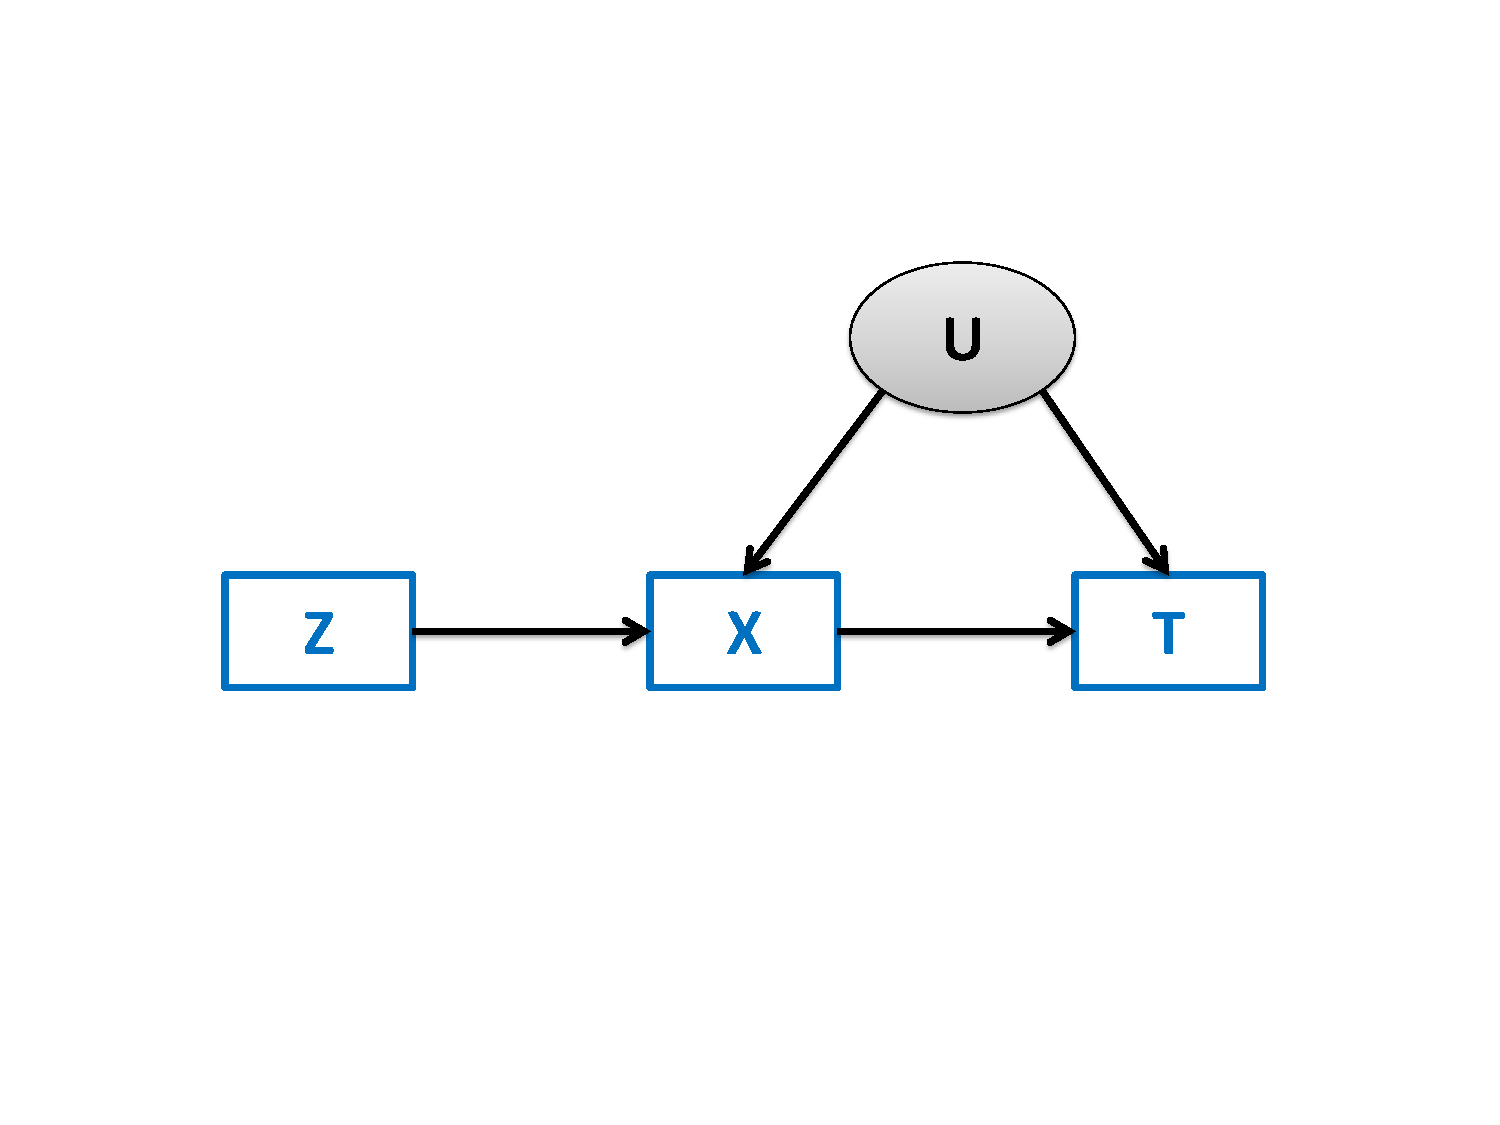
\includegraphics[width=1.05\onecolwid]{Figs/IV.pdf}}}

    \end{block}

  \colonevsepsmall% between blocks


    \begin{block}{Rank-based estimator for the standard AFT model}{

	\begin{align*}
	U_n(\beta) &= \sum_{i = 1}^n\int \rho(t, \beta)\{ X_i - \oline{X}(t, \beta) \} \mbox{ } \mathrm{d}N_i(t, \beta) \\
	& \\	
	 \mbox{where } \oline{X}(t, \beta) &\equiv 
	\frac{1}{n}\sum_{j=1}^n X_j I(\epsilon_j^\beta \ge t) \mbox{ } / \mbox{ } \frac{1}{n}\sum_{j=1}^n I(\epsilon_j^\beta \ge t) \mbox{  and} \\
	\epsilon_i^\beta &= \log{T_i} - \beta X_i \mbox{ is the residual for subject }i \mbox{ and }\\
	N_i(t, \beta) &= I(\epsilon_i^\beta \leq t, \Delta_i = 1)
	\end{align*}

    }
    \end{block}

\colonevsepsmall

    \begin{exampleblock}{\Large Rank-based   IV estimator for the AFT model}

	{\hilit Key Difference:} instead of comparing $X_i$ with the average $X$ in the residual risk set, we compare $Z_i$ with the average $Z$ in the residual risk set

	\begin{align*}
	U_n^{IV-IPCW}(\beta) &= \sum_{i = 1}^n\int \rho(t, \beta)\{ {\color{Blue}Z_i} - {\color{Blue}\oline{Z}_{G_C}(t, \beta)} \} \frac{\mathrm{d}N_i(t, \beta)}{G_C(t + \beta X_i)} \\
	& \\
	 \mbox{where } {\color{Blue}\oline{Z}_{G_C}(t, \beta)} &\equiv 
	\frac{1}{n}\sum_{j=1}^n \frac{{\color{Blue}Z_j} I({\color{Blue}\epsilon_j^\beta} \ge t)}{G_C(t + \beta X_j)} \mbox{ } / \mbox{ } 
	\frac{1}{n}\sum_{j=1}^n \frac{I(  {\color{Blue}\epsilon_j^\beta} \ge t)}                  {G_C(t + \beta X_j)} \mbox{  and} \\
	{\color{Blue}\epsilon_i^\beta} &= \log{T_i} - \beta {\color{Blue}X_i} \mbox{ is the residual for subject } i 
	& \\
	&\mbox{and } G_C \mbox{ is the Kaplan-Meier estimator for the} \\ 
	&\mbox{survival} \mbox{ function of } C
	\end{align*}

	We need to use inverse probility of censoring weighting to account for induced dependence of $C_i$ on $\epsilon_i^\beta$
    \end{exampleblock}



  \end{column}


  \begin{column}{\sepwid} \end{column} % empty spacer column


  \begin{column}{\onecolwid}

    \begin{exampleblock}{\Large Inference via Bootstrap}

	{\hilit Challenge:} Too computationally demanding to resample the data and solve a resampled equation many times

	{\hilit Instead:} Relate the variance of $\sqrt{n}(\hat{\beta} - \beta)$ to the variance of $n^{-1/2}U_n^{IV-IPCW}(\beta) $

	The approach of \citep{zeng08} only involves evaluations of the estimating equation


    \end{exampleblock}

  \colonevsepsmall % between blocks

    \begin{block}{\Large Simulation}{
    %\begin{minipage}[t]{\halfcolwid}
    \vspace*{0mm}

    \bi
    \item $T = \exp{\{ X + \beta_U U + \epsilon \}}$ \\
	where
    \item $X = \alpha_Z \exp{\{Z\}} + \alpha_U U + \epsilon^* $ where $\epsilon$, $\epsilon^* \sim N(0,1)$, $\epsilon \perp\!\!\!\perp \epsilon^*$
    \item $C \sim $ exponential with rate parameter 1
    \ei

    \vspace{8pt}

           %$\alpha_U$ and $\beta_U$ characterize the strength of unmeasured confounding

          % \vspace{5pt}

          %$\alpha_Z$ characterizes the strength of the instrumental variable

	\vspace{5pt}

	Nonlinearity between $Z$ and $X$ to demonstrate structural \\ assumptions not necessary
	\vspace{25pt}

Two other methods investigated:

    \bi
    \item Rank-based IV estimator  without inverse weighting (not theoretically justified)
    \item Two stage procedure; replace $X$ with predictions of $X$ using linear model with $Z$
    \ei


    %\end{minipage}
    %\hfill
    %\begin{minipage}[t]{\halfcolwid}
    %\vspace*{0mm}

   %% \includegraphics[width=\halfcolwid]{Figs/gravitropism.png}

    %\end{minipage} 
    }
   %%%%%%%%%%%  \end{block}


   %%%%%%%%%%% \colonevsepsmall % between blocks

   %%%%%%%%%%% \begin{block}{Results}

    \vspace{50pt}

	\centerline{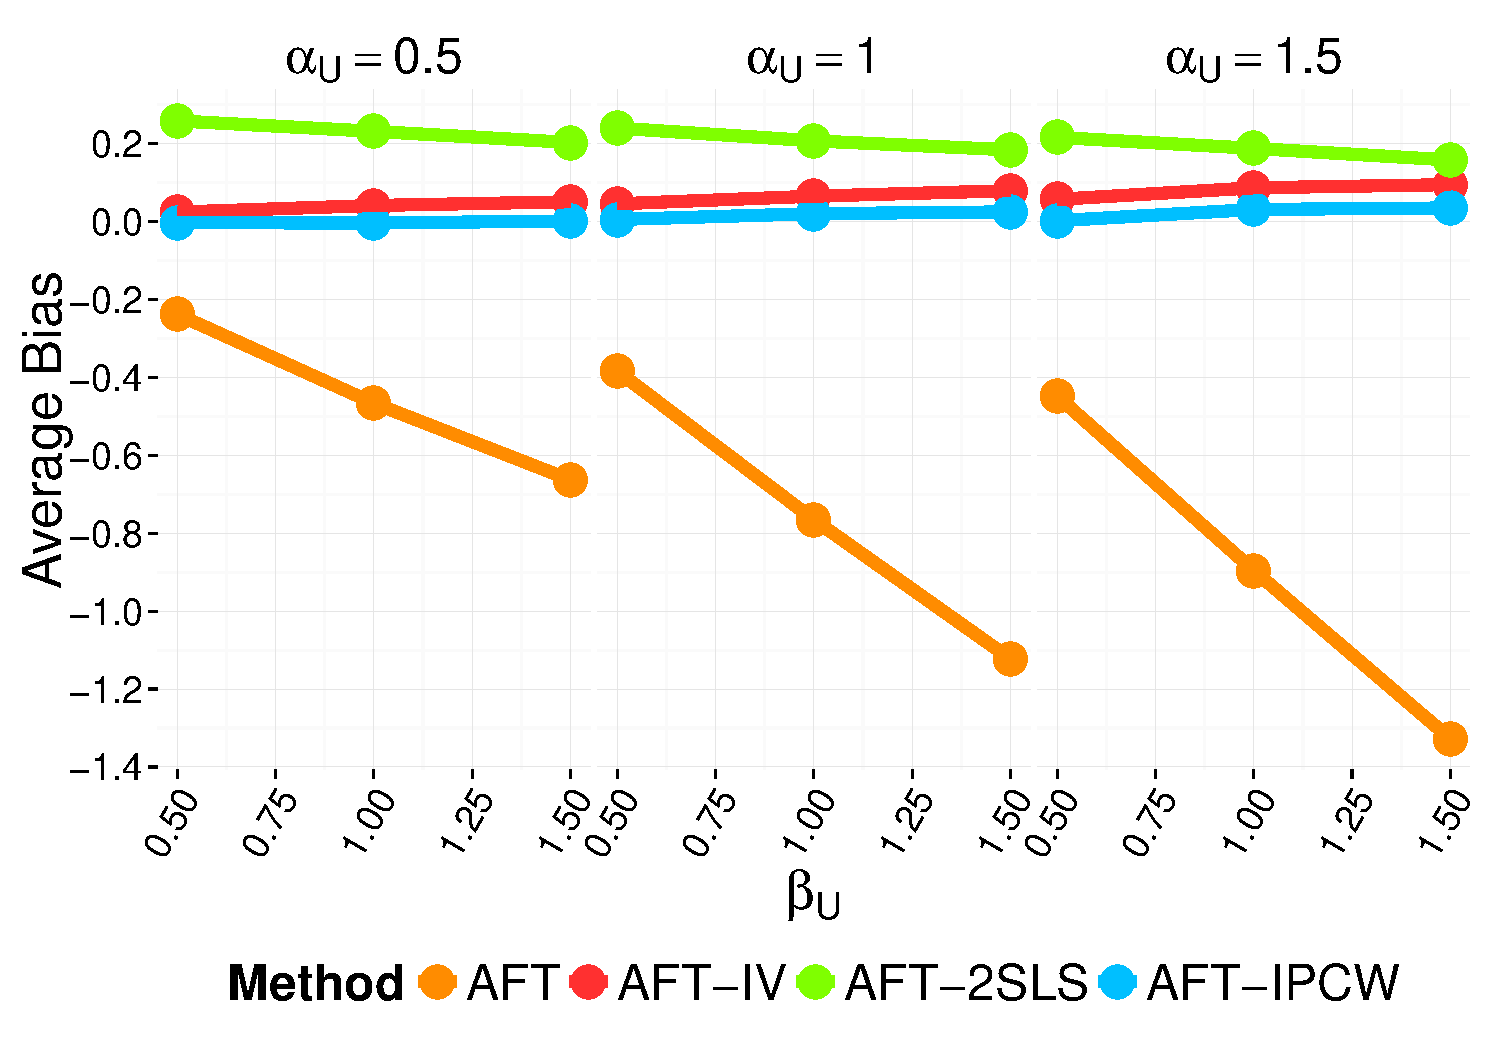
\includegraphics[width=0.95\onecolwid]{Figs/beta_u_over_alpha_u.pdf}}

	%\centerline{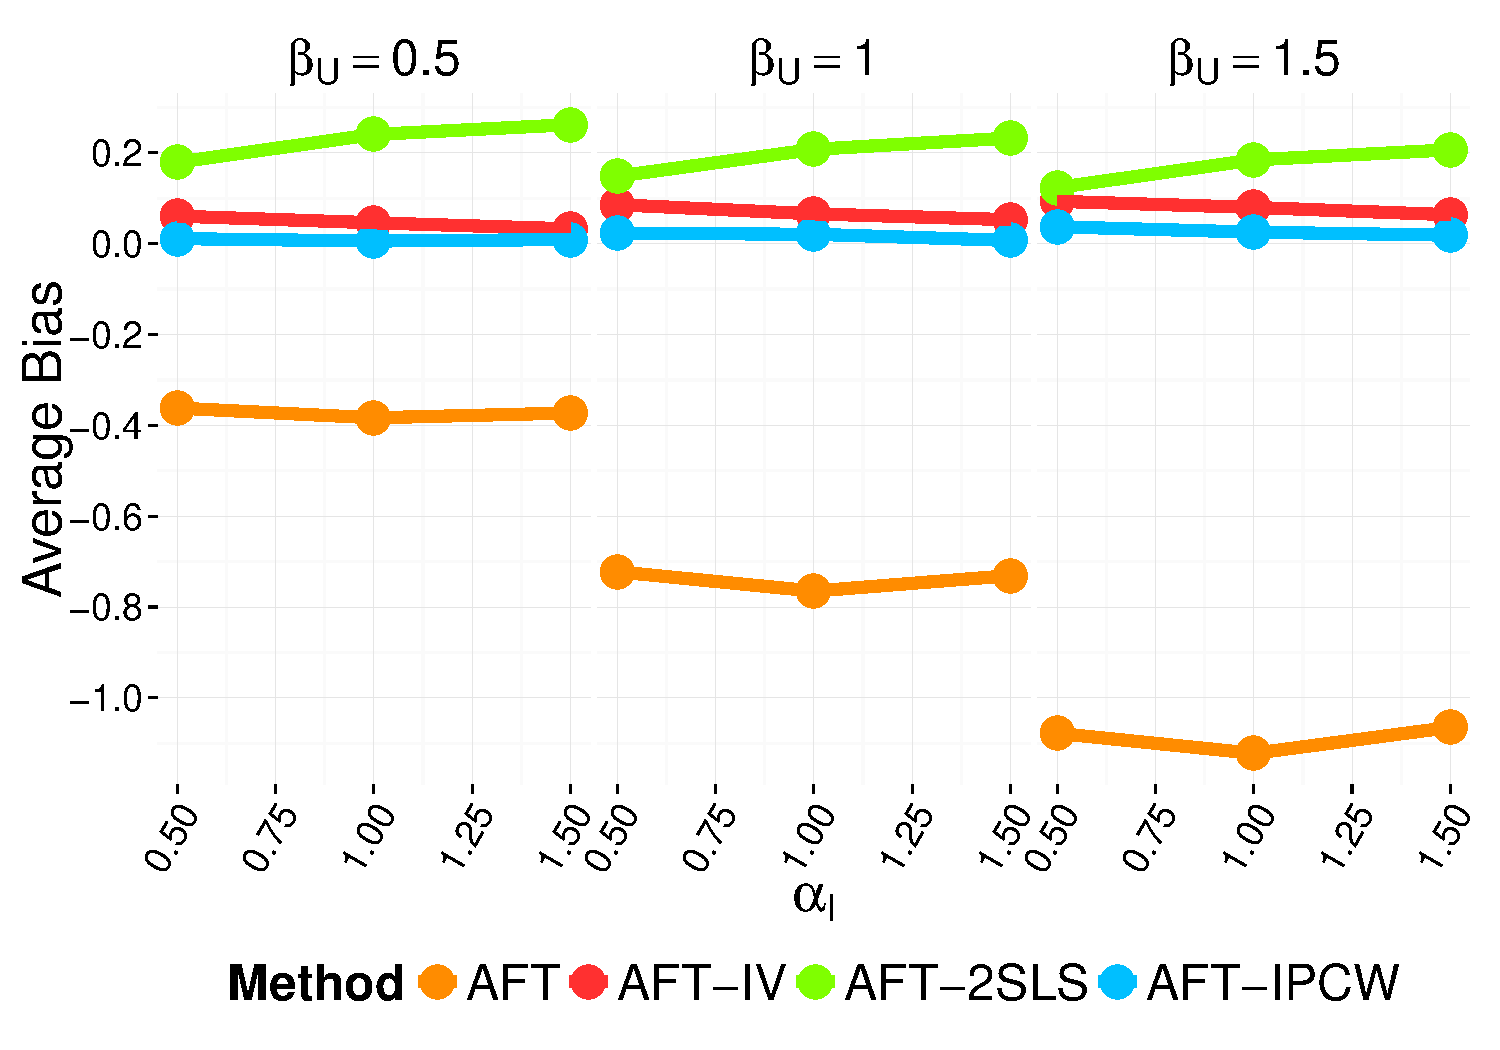
\includegraphics[width=1.01\onecolwid]{Figs/alpha_I_over_beta_u.pdf}}

    \vspace{40pt}
\newcolumntype{y}{>{\columncolor{LightYellow}}c}
\newcolumntype{d}{>{\columncolor{darkorange}}c}
\newcolumntype{f}{>{\columncolor{firebrick1}}c}
\newcolumntype{g}{>{\columncolor{chartreuse}}c}
\newcolumntype{b}{>{\columncolor{deepskyblue1}}c}


	\begin{table}\label{simulation}
\centering
\begin{tabular}{@{}lllccccccbb@{}}
\midrule
& & & \multicolumn{2}{c}{AFT} & \multicolumn{2}{c}{AFT IV} & \multicolumn{2}{c}{AFT 2SLS} & \multicolumn{2}{c}{AFT IPCW} \\ 
& & & \multicolumn{2}{c}{Sample Size} & \multicolumn{2}{c}{Sample Size} & \multicolumn{2}{c}{Sample Size} & \multicolumn{2}{c}{Sample Size} \\ 
$\alpha_u$ & $\beta_u$ & $\alpha_I$ & \multicolumn{1}{c}{500} & \multicolumn{1}{c}{5000} & \multicolumn{1}{c}{500} & \multicolumn{1}{c}{5000} & \multicolumn{1}{c}{500} & \multicolumn{1}{c}{5000} & \multicolumn{1}{c}{500} & \multicolumn{1}{c}{5000} \\ 
\midrule
0.5 & 0.5 & 0.5  & $0.542$ & $0.000$ & $0.848$ & $0.874$ & $0.902$ & $0.296$ & $0.928$ & $0.970$ \\
 &  & 1  & $0.742$ & $0.026$ & $0.844$ & $0.920$ & $0.762$ & $0.012$ & $0.936$ & $0.970$ \\
% &  & 1.5  & $0.820$ & $0.174$ & $0.870$ & $0.928$ & $0.684$ & $0.002$ & $0.930$ & $0.958$ \\
 & 1 & 0.5  & $0.100$ & $0.000$ & $0.838$ & $0.852$ & $0.912$ & $0.544$ & $0.924$ & $0.938$ \\
 &  & 1  & $0.422$ & $0.000$ & $0.880$ & $0.888$ & $0.842$ & $0.086$ & $0.906$ & $0.966$ \\
% &  & 1.5  & $0.632$ & $0.000$ & $0.898$ & $0.890$ & $0.780$ & $0.032$ & $0.906$ & $0.952$ \\
\midrule
1 & 0.5 & 0.5  & $0.146$ & $0.000$ & $0.798$ & $0.858$ & $0.938$ & $0.638$ & $0.910$ & $0.960$ \\
 &  & 1  & $0.406$ & $0.000$ & $0.840$ & $0.866$ & $0.808$ & $0.050$ & $0.924$ & $0.968$ \\
% &  & 1.5  & $0.584$ & $0.002$ & $0.882$ & $0.866$ & $0.738$ & $0.004$ & $0.948$ & $0.954$ \\
 & 1 & 0.5  & $0.002$ & $0.000$ & $0.826$ & $0.774$ & $0.964$ & $0.808$ & $0.920$ & $0.948$ \\
 &  & 1  & $0.054$ & $0.000$ & $0.856$ & $0.786$ & $0.872$ & $0.184$ & $0.906$ & $0.938$ \\
% &  & 1.5  & $0.196$ & $0.000$ & $0.862$ & $0.880$ & $0.828$ & $0.060$ & $0.928$ & $0.938$ \\
\bottomrule 
\end{tabular}
	\caption{Empirical Coverage, 95\% Level. Simulations based on 500 simulated datasets, 1000 bootstrap replications}
	\end{table}

    \end{block}



  \end{column}

  \end{columns}
  \end{column}

\begin{column}{\sepwid} \end{column}                 % empty spacer column

  \begin{column}{\twocolwid}
    \begin{exampleblock}{\Large Analysis of Medicare Enrollment Data}{
    \begin{center}
    \begin{minipage}[t]{0.7\onecolwid}
    \vspace*{0mm}

    \bi
    \item Approximately 100k patients
    \item Approximately 44k  deaths
    \item Surgeries performed between 2001 and 2008 and followed up until 2009
    \ei

    \end{minipage}
    \hspace{0.5\sepwid}
    \begin{minipage}[t]{0.8\onecolwid}
    \vspace*{0mm}

    \bi
    \item Data includes 2,853 cases of abdominal aortic rupture
    \item Primary outcome is all-cause survival time
    \item Demographic information as well as medical information, including chronic conditions
    \ei

    \end{minipage} \end{center}
    }
    \end{exampleblock}

    \vspace{1mm} % between blocks

    \begin{columns}[t]

      \begin{column}{\onecolwid}

       % \href{http://www.biostat.wisc.edu/~kbroman/posters/ENAR2014/1a}{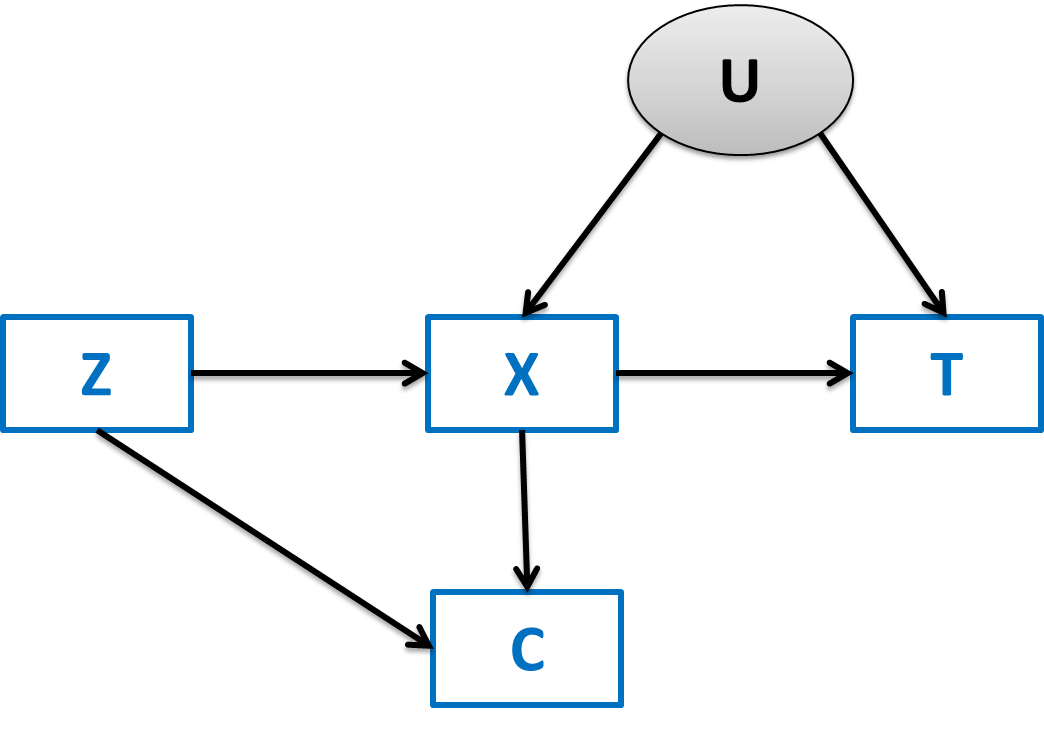
\includegraphics[width=2cm]{Figs/IV1.png}}

       %\centerline{\href{http://www.biostat.wisc.edu/~kbroman/posters/ENAR2014/1a}{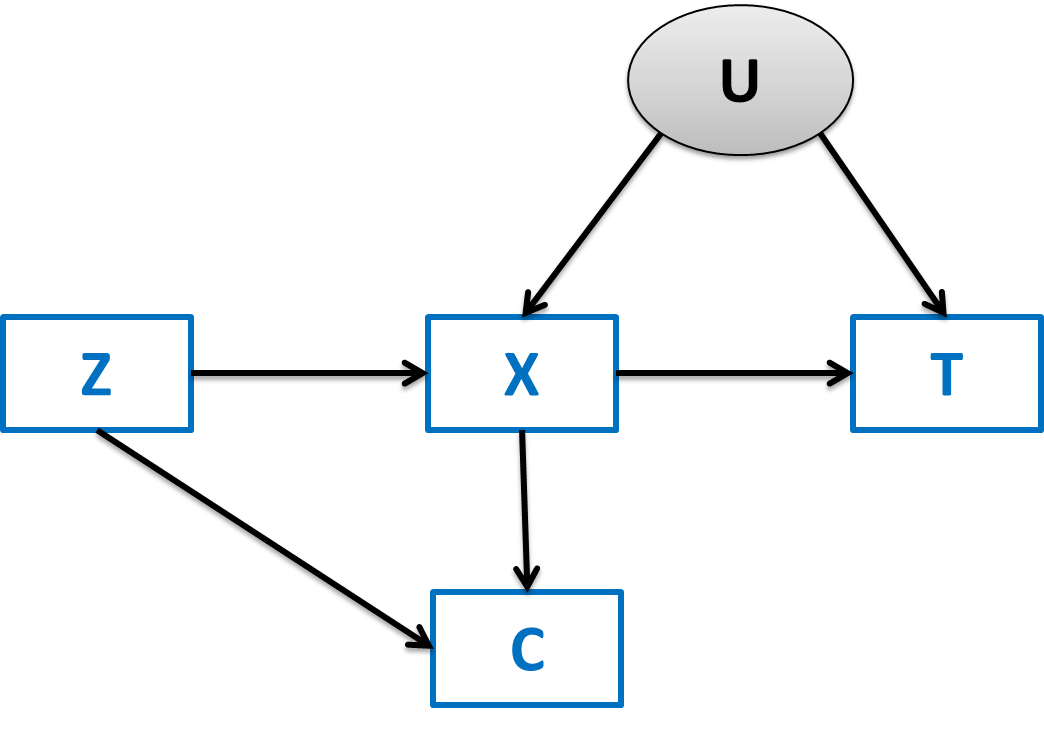
\includegraphics[width=\onecolwid]{Figs/IV1.png}}}

      \vspace{10mm} % after legend

        \begin{exampleblock}{} \rmfamily %[sep=1em, wd=1.0\onecolwid]{legend}
	   \bi
	      \item {\bluebold \large  AAA Background}
	          \vspace{8pt}
	         \bi \itemsep14pt
	         \item Randomized controlled trials suggest 
			\bi
				\item a short term mortality reduction for EVAR (Prinssen et al., 2004) 
				\item little difference long-term (Lederle et al., 2012)
			\ei
	         \item Observational studies utilizing propensity score-matched cohorts \citep{schermerhorn08} suggest
			\bi
				\item EVAR has short-term benefits
				\item older patients benefit more from EVAR
				\item reinterventions are more common after EVAR 
			\ei
	         \ei

		\vspace{24pt}
	      \item {\bluebold \large Instrumental variable}
	          \vspace{8pt}
	         \bi \itemsep14pt
	         \item Proportion of EVAR surgeries to open surgeries at the institution in which the patient received treatment
	         \item Predictive of actual surgery received, indicating moderate instrument strength
	         \item {\hilit Potential weaknesses:} 
			\bi
				\item possibly institutions which perform one type of surgery often see more ill patients
				\item institutions which perform one type of surgery more often could perform them better than other institutions
			\ei
	         \ei
 	     \ei
        \end{exampleblock}


    \colsevenvsep % between blocks

    \begin{exampleblock}{\Large Analysis}

	{\bluebold \large Four approaches:}

	\vspace{8pt}

	         \bi \itemsep14pt
	           \item Standard AFT
	           \item AFT with IV and no inverse probability of censoring weighting
	           \item AFT two stage procedure (analogous to 2SLS)
	           \item AFT with IV and inverse probability of censoring weighting (our proposed method)
	         \ei


    \end{exampleblock}

    \colsevenvsep % between blocks

    \begin{exampleblock}{\Large Estimates of EVAR Effect}

	\vspace{8pt}

	

	\begin{table}\label{analysis}
	\centering
	\begin{tabular}{@{} lSSS @{}}\toprule
		{Estimator} & {$\bm\hat{\boldsymbol\beta}_{EVAR}$} & {(95\% Conf.} & {Interval)} \\ \midrule
		AFT & 0.047 & -0.063 & 0.144 \\
		AFT-IV & -0.169 & -0.420 & 0.080 \\
		AFT-2SLS & -0.175 & -0.432 & 0.074 \\
		AFT-IV-IPCW  & -0.156 &  -0.364 & 0.052  \\
	\bottomrule
	\end{tabular}
	\caption{Estimates of the effect of EVAR vs. open repair for rupture cases }
	\end{table}

	

    \end{exampleblock}


      \end{column}

      \begin{column}{\sepwid} \end{column} % empty spacer column

      \begin{column}{\onecolwid}

      \vspace{10mm} % after legend

    \begin{exampleblock}{\Large Conclusions}

	\vspace{8pt}

	         \bi \itemsep14pt
	           \item Analysis adjusting for unmeasured confounding suggests there may be some benefit for open repair for rupture cases
		\item Suggests that more comprehensive treatment provided by open repair leads to reduction in mortality for more serious AAA cases
	           \item Rupture cases are more serious than typical AAA cases; conclusion may be different for non-rupture cases
		\item Our analysis is consistent with a recent study of ruptured AAA which provides sensitivity analysis to bias due to unmeasured confounding \citep{edwards14}
	         \ei


    \end{exampleblock}


  \colonevsep % between blocks

    \begin{block}{\Large Remaining Challenges }{
      \bi
      \itemsep18pt
      \item Our estimating equation is not monotone and often has poor behavior in small samples
	\bi
		\item Monotonicity would also improve computation dramatically
		\item Could alleviate difficulties in analyzing entire dataset
	\ei
      \item Sensitivity of the bootstrap procedure 
      \ei
    }
    \end{block}

  \colonevsep % between blocks

    \begin{block}{Contact}
      %\hspace{0.5em}
	\noindent
        \begin{minipage}[t]{0.9\halfcolwid}
        \href{http://www.stat.wisc.edu/~huling}{Jared Huling}\\
        {\tt huling@wisc.edu}\\
        \href{http://www.stat.wisc.edu/~huling}{\tt www.stat.wisc.edu/{\textasciitilde}huling} \\
        \end{minipage}
\hfill
      \hspace{-1em}
	\noindent
        \begin{minipage}[t]{0.95\halfcolwid}
        \href{http://www.biostat.wisc.edu/content/yu-menggang}{Menggang Yu}\\
        {\tt meyu@biostat.wisc.edu}\\
        \end{minipage}


    \end{block}

      \begin{block}{References} 

        {\small 
	%\setbeamertemplate{bibliography item}[text]
	\bibliographystyle{plainnat} 
       	\bibliography{references}
         } 
      \end{block} 

    \vspace{40pt}
    {\rmfamily \footnotesize
    \centerline{This work was supported in part by NIH grant T32HL083806.}}

    \vspace{10pt}
    {\rmfamily \footnotesize
    \centerline{Thanks to Karl Broman for the poster template \href{https://github.com/kbroman/Poster_ENAR2014}{github.com/kbroman/Poster\_ENAR2014}}}


      \end{column}
  \end{columns}
  \end{column}


  \begin{column}{\sepwid}\end{column} % empty spacer column

\end{columns}

%\hrule   % <- uncomment to help check that the columns are the same length

\end{frame}

\end{document}
